\documentclass{article}
\usepackage[utf8]{inputenc}
\usepackage[margin=1in]{geometry}

\title{LCA and $2^n$ Jump Pointers}
\author{Larry Wang }
\date{October 21 2016}

\usepackage{float}
\usepackage{tikz}
\usetikzlibrary{calc,shapes.multipart,chains,arrows,positioning}

\definecolor{myseagreen}{RGB}{230,250,250}
\tikzstyle{vertex}=[draw,fill=myseagreen,circle,minimum size=24pt,inner sep=0pt]

\begin{document}

\maketitle

\section{Introduction}
If we are given an undirected graph $G$ that contains no cycles, then we may designate any one of its vetices as the root. By rooting the tree, we give all of the edges the natural direction of pointing towards the root. Additionally, we can define the height of a vertex as its distance to the root. The LCA, or Lowest Common Ancestor, problem involves finding the node of maximum height that is an ancestor of two given nodes. 

\begin{figure}[H]
\centering
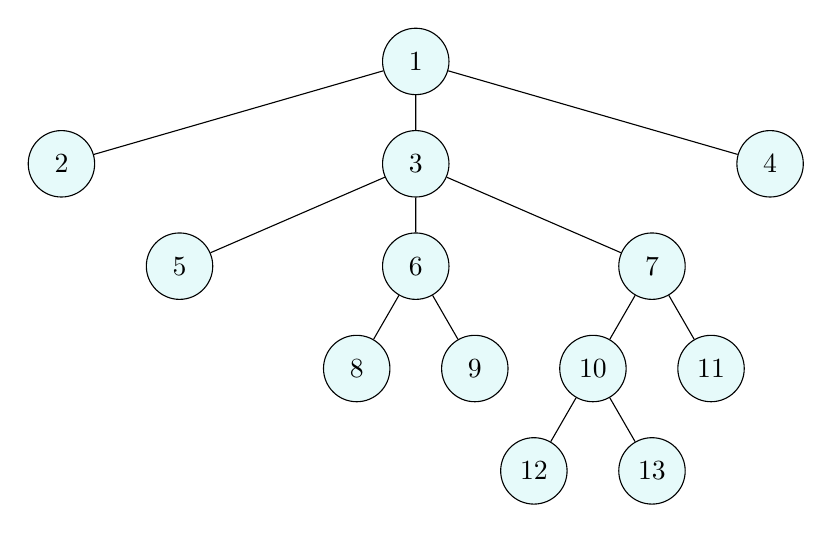
\begin{tikzpicture}[level/.style={sibling distance=15mm,level distance=13mm}]
\node [vertex] {1}
  child [sibling distance=45mm] {
    node [vertex] {2}
  }
  child [sibling distance=45mm] {
    node [vertex] {3}
    child [sibling distance=30mm] { 
        node [vertex] {5} 
    }
    child [sibling distance=30mm]{
      node [vertex] {6}
      child { node [vertex] {8} }
      child { node [vertex] {9} }
    }
    child [sibling distance=30mm] {
      node [vertex] {7}
      child {
        node [vertex] {10}
        child { node [vertex] {12} }
        child { node [vertex] {13} }
      }
      child { 
        node [vertex] {11} 
      }
    }
  }
  child [sibling distance=45mm] {
    node [vertex] {4}
  };
\end{tikzpicture}
\end{figure}


\section{DFS}

Before we begin finding the LCA, it is in our best interest to be able to calculate the height of each node (for reasons that will become apparent later). To do this, we can simply do a DFS starting at the root. This has complexity $O(N)$. 


\section {Naive Solution}

Supposed we want to find the LCA of nodes $u$ and $v$ such that $h(u)>h(v)$. Notice that the LCA cannot be any node with height greater than $h(v)$, so we repeatedly reassign $u$ with its parent until $u$ and $v$ have the same height. Now, we repeatedly reassign both $u$ and $v$ to their parents until they point to the same node. This node is the LCA of $u$ and $v$. This algorithm is equivalent to moving $u$ and $v$ one level up at a time until they match.

Note that this has worst case time complexity $O(N)$. This occurs when the tree is effectively a linked list. Additionally, this algorithm requires $O(N)$ preprocessing because we must calculate the heights of each node. Unfortunately, many problems will require us to perform multiple LCA queries, so $O(N)$ is too slow. 


\section {Another Naive Solution}

Realizing that the bottleneck of the previous solution was in querying, we now take a different approach: solely preprocessing. Instead of calculating the LCAs query by query, we instead calculate the LCA of all pairs of nodes beforehand. Note that this has complexity $O(N^3)$ (why?), but we can use dynamic programming to reduce this to $O(N^2)$. Now, our query time is $O(1)$, but $O(N^2)$ preprocessing is still undesirable. 


\section {$2^n$ Jump Pointers}

Based on the previous two solutions, we would now like to develop an algorithm that balances both preprocessing and query time. Consider the $N \times \log N$ table $A$, where $A(i, j)$ represents the node that is $2^j$ steps above node $i$. We can compute the contents of the table with the following dynamic programming formulation: 
$$A(i, 0) = parent(i)$$
$$A(i, j+1) = A( A(i, j), j )$$

\noindent The recurrence relation is analogous to first moving $2^j$ steps to node $A(i, j)$, and then moving an additional $2^j$ steps to traverse a total of $2^{j+1}$ steps above $i$. Thus, $A$ can be computed in $O(N \log N)$. 

Now, to actually find the LCA of $u$ and $v$, we employ a similar approach taken in the first Naive Solution, but using our $2^n$ jump pointer table. Assume $h(u) > h(v)$ and let $d = h(u) - h(v)$ be the difference in height. Note that $d$ can be written as a sum of at most $\log d$ unique powers of 2 (Hint: consider the binary representation of $d$). Since $A$ tells us how to move nodes upwards in increments of powers of two, this means that $u$ can be moved $d$ steps upwards by making $\log d$ lookups in $A$. Once $u$ and $v$ are at the same height, we repeatedly move them upwards by the largest power of 2 such that $u$ and $v$ do not point to the same node. This works because if $A(u, i) \neq A(v, i)$, then $LCA(u, v) = LCA(A(u, i), A(v, i))$. In this manner, we can repeatedly reduce the distance from $u$ and $v$ to $LCA(u, v)$ by a factor of at least two.  Thus, this takes $O(\log N)$ lookups in $A$, so the complexity of each LCA query is $O(\log N)$. 


%find me more problems pls
\section {Problems}

\begin{enumerate}
    \item USACO December 2015, Platinum Contest Problem 1, Max Flow
    \item Codeforces 702E Analysis of Pathes in Functional Graph
    \item Sort an array containing all $n-1$ suffixes of a string of length $n$ (This data structure is called a Suffix Array and can be used to answer string search queries in $O(\log N)$). 
\end{enumerate}

\end{document}
